\section{Αρχιτεκτονικές Νευρωνικών Δικτύων}
\noindent

Ο όρος \textit{'αρχιτεκτονική ANN'} αναφέρεται στην διάταξη των νευρώνων σε επίπεδα, τις συνδέσεις μεταξύ των επιπέδων, τις συναρτήσεις ενεργοποίησης και τις μεθόδους μάθησης \cite{Kalogirou_2014}. Απλούστερα, γίνεται σαφές ότι αναφέρεται στο σύνολο της κατασκευής ενός NN. Το \textit{μοντέλο} του ΝΝ, και η αρχιτεκτονική του, καθορίζουν τον τρόπο που η είσοδος παράγει με υπολογιστικό τρόπο μια έξοδο. Η βασική λειτουργία που πρέπει να ακολουθηθεί για την σωστή αντιμετώπιση ενός προβλήματος, είναι όπως φαίνεται, αυτή της επιλογής της σωστής αρχιτεκτονικής καθώς και των υπερπαραμέτρων που αναλύονται στην υποενότητα \ref{subsub:hyperparameters}. Εξίσου σημαντική, είναι η επιλογή της αντικειμενικής συνάρτησης, η οποία συχνά αποκαλείται και συνάρτηση απώλειας (loss function), που είναι επιθυμητό να ελαχιστοποιηθεί (ή να μεγιστοποιηθεί αναλόγως με το πρόβλημα). Σε αυτή την εργασία, τα μοντέλα προσπαθούν να ελαχιστοποιήσουν το \textit{Μέσο Τετραγωνικό Σφάλμα} (MSE), ενώ κατά την εκπαίδευσή τους παρακολουθείται το Μέσο Απόλυτο Σφάλμα (MAE) και η Ρίζα του Μέσου Τετραγωνικού Σφάλματος (RMSE). Δοκιμάστηκε η απόδοση αρκετών διαφορετικών μοντέλων, εδώ όμως αναλύονται τα καλύτερα εκ των δύο ευρύτερων κατηγοριών, των πλήρως διασυνδεδεμένων (Fully Connected), και των συνελικτικών (Convolutional). Εδώ σημειώνεται πως η προεπεξεργασία των δεδομένων, καθώς και τα ίδια τα μοντέλα έχουν υλοποιηθεί με τη βοήθεια της βιβλιοθήκης TensorFlow στη γλώσσα Python. Στο πακέτο αυτό προστέθηκαν μερικές custom συναρτήσεις για την λεπτομερέστερη παρακολούθηση του χρόνου εκτέλεσης.

\subsection{Fully Connected}
Το πλήρως διασυνδεδεμένο μοντέλο που έδωσε τα καλύτερα αποτελέσματα, απεικονίζεται στο Σχήμα \ref{fig:FC_Arch}, και αποτελείται από ένα επίπεδο εισόδου με 71276 νευρώνες, τέσσερα κρυφά επίπεδα με 2000, 360, 180 και 90 νευρώνες αντίστοιχα, καθώς και το επίπεδο εξόδου, που έχει έναν νευρώνα που δίνει την πρόβλεψη. Μετά το επίπεδο εισόδου, καθώς και μετά από το 1ο κρυφό επίπεδο, τοποθετείται ένα επίπεδο Dropout, το οποίο δεν αποτελείται από νευρώνες, αλλά ελέγχει τους νευρώνες του προηγούμενου επιπέδου. Όλα τα επίπεδα που περιέχουν νευρώνες, χρησιμοποιούν την ReLU (εξίσωση \ref{eq:ReLU}) ως συνάρτηση ενεργοποίησης.

Αναλυτικότερα, η εκπαίδευση έγινε χρησιμοποιώντας, όπως έχει ήδη αναφερθεί, ως συνάρτηση απώλειας το MSE, και τον βελτιστοποιητή Adam (Adaptive Moment Estimation) με αρχικό ρυθμό μάθησης $Lr = 0.001$. 

\begin{figure}[h]
\centering
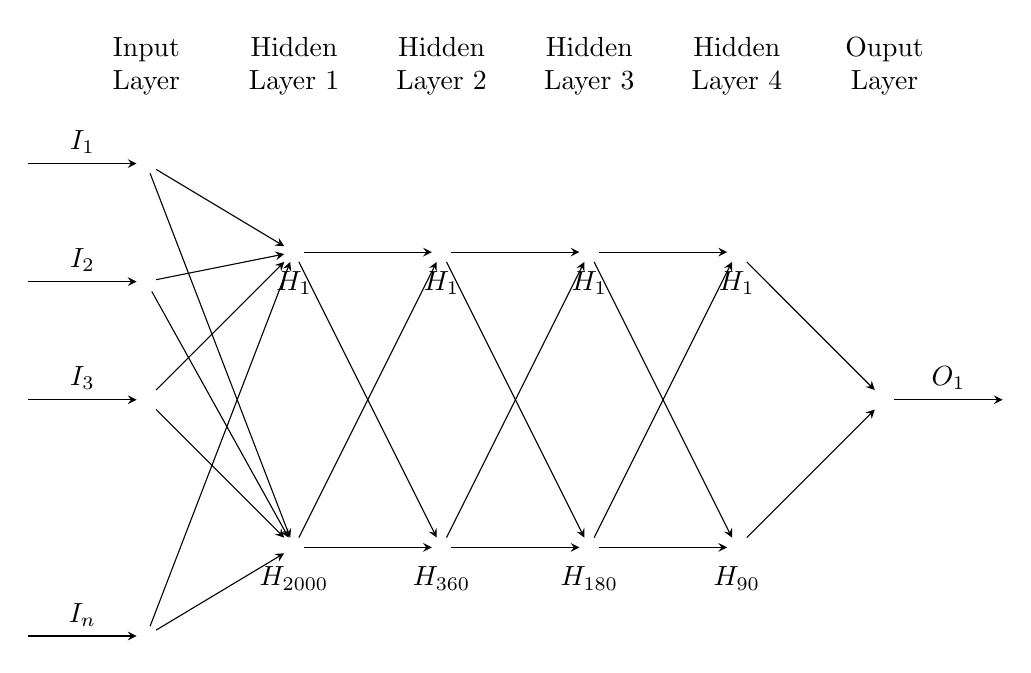
\begin{tikzpicture}[x=1.5cm, y=1.5cm, >=stealth]

\foreach \m/\l [count=\y] in {1,2,3,missing,4}
  \node [every neuron/.try, neuron \m/.try] (input-\m) at (0,2.5-\y) {};

\foreach \m [count=\y] in {1,missing,2}
  \node [every neuron/.try, neuron \m/.try ] (1-hidden-\m) at (1.25,2-\y*1.25) {};

\foreach \m [count=\y] in {1,missing,2}
  \node [every neuron/.try, neuron \m/.try ] (2-hidden-\m) at (2.5,2-\y*1.25) {};
  
 \foreach \m [count=\y] in {1,missing,2}
  \node [every neuron/.try, neuron \m/.try ] (3-hidden-\m) at (3.75,2-\y*1.25) {};

\foreach \m [count=\y] in {1,missing,2}
  \node [every neuron/.try, neuron \m/.try ] (4-hidden-\m) at (5,2-\y*1.25) {};
  
  
\foreach \m [count=\y] in {1}
  \node [every neuron/.try, neuron \m/.try ] (output-\m) at (6.25,\y-1.5) {};

\foreach \l [count=\i] in {1,2,3,n}
  \draw [<-] (input-\i) -- ++(-1,0)
    node [above, midway] {$I_\l$};

\foreach \l [count=\i] in {1,2000}
  \node [below] at (1-hidden-\i.south) {$H_{\l}$};
  
  \foreach \l [count=\i] in {1,360}
  \node [below] at (2-hidden-\i.south) {$H_{\l}$};

\foreach \l [count=\i] in {1,180}
  \node [below] at (3-hidden-\i.south) {$H_{\l}$};

\foreach \l [count=\i] in {1,90}
  \node [below] at (4-hidden-\i.south) {$H_{\l}$};
  
  
\foreach \l [count=\i] in {1}
  \draw [->] (output-\i) -- ++(1,0)
    node [above, midway] {$O_\l$};

\foreach \i in {1,...,4}
  \foreach \j in {1,...,2}
    \draw [->] (input-\i) -- (1-hidden-\j);

\foreach \i in {1,...,2}
  \foreach \j in {1,...,2}
    \draw [->] (1-hidden-\i) -- (2-hidden-\j);

\foreach \i in {1,...,2}
  \foreach \j in {1,...,2}
    \draw [->] (2-hidden-\i) -- (3-hidden-\j);

\foreach \i in {1,...,2}
  \foreach \j in {1,...,2}
    \draw [->] (3-hidden-\i) -- (4-hidden-\j);

    
\foreach \i in {1,...,2}
  \foreach \j in {1}
    \draw [->] (4-hidden-\i) -- (output-\j);

\foreach \l [count=\x from 0] in {Input\\Layer, Hidden\\Layer 1, Hidden\\Layer 2, Hidden\\Layer 3, Hidden\\Layer 4, Ouput\\Layer}
  \node [align=center, above] at (\x*1.25,2) {\l};

\end{tikzpicture}
\caption{Fully connected χωρίς τα επίπεδα Dropout.}
\label{fig:FC_Arch}
\end{figure}

\subsubsection{Επίπεδο Dropout}
Με απλά λόγια, η λειτουργία του επιπέδου Dropout, είναι η απενεργοποίηση, με τυχαίο τρόπο, νευρώνων του προγηούμενου επιπέδου. Το επίπεδο αυτό, έχει μία υπερπαράμετρο, το \textit{Dropout Rate} (DR), το οποίο καθορίζει το πλήθος των νευρώνων που απενεργοποιούνται σε κάθε εποχή (ένα πέρασμα ολόκληρου του dataset από το νευρωνικό). Για παράδειγμα, για $DR=0.4$, με το προηγούμενο επίπεδο να έχει 2000 νευρώνες, σε κάθε εποχή απενεργοποιούνται οι $2000*0.4 = 800$ από αυτούς. Το αποτέλεσμα αυτής της διαδικασίας, είναι το νευρωνικό να μην βασίζεται αποκλειστικά σε μερικούς νευρώνες εκ του συνόλου για την τελική εκτίμηση που δίνει στην έξοδο μειώνοντας με αυτόν τον τρόπο σημαντικά το overfitting. Μια συνοπτική περιγραφή της λειτουργίας του επιπέδου, φαίνεται στο Σχήμα \ref{fig:dropout_ex}. Σε αυτό το σχήμα θεωρείται πως υπάρχει ένα Dropout Layer ενδιάμεσα από όλα τα επίπεδα.

\begin{figure}
\centering
\scalebox{.8}{
\hbox{\hspace{-2em}
\begin{tikzpicture}

	\node[circle, draw, thick] (i1) {};
	\node[circle, draw, thick, above=2em of i1] (i2) {};
	\node[circle, draw, thick, above=2em of i2] (i3) {};
	\node[circle, draw, thick, below=2em of i1] (i4) {};
	\node[circle, draw, thick, below=2em of i4] (i5) {};
	
	\node[circle, draw, thick, right=4em of i1] (h1) {};
	\node[circle, draw, thick, right=4em of i2] (h2) {};
	\node[circle, draw, thick, right=4em of i3] (h3) {};
	\node[circle, draw, thick, right=4em of i4] (h4) {};
	\node[circle, draw, thick, right=4em of i5] (h5) {};
	
	\node[circle, draw, thick, right=4em of h1] (hh1) {};
	\node[circle, draw, thick, right=4em of h2] (hh2) {};
	\node[circle, draw, thick, right=4em of h3] (hh3) {};
	\node[circle, draw, thick, right=4em of h4] (hh4) {};
	\node[circle, draw, thick, right=4em of h5] (hh5) {};
	
	\node[circle, draw, thick, right=4em of hh2] (o1) {};
	\node[circle, draw, thick, right=4em of hh4] (o2) {};
	
	\draw[-stealth, thick] (i1) -- (h1);
	\draw[-stealth, thick] (i1) -- (h2);
	\draw[-stealth, thick] (i1) -- (h3);
	\draw[-stealth, thick] (i1) -- (h4);
	\draw[-stealth, thick] (i1) -- (h5);
	\draw[-stealth, thick] (i2) -- (h1);
	\draw[-stealth, thick] (i2) -- (h2);
	\draw[-stealth, thick] (i2) -- (h3);
	\draw[-stealth, thick] (i2) -- (h4);
	\draw[-stealth, thick] (i2) -- (h5);
	\draw[-stealth, thick] (i3) -- (h1);
	\draw[-stealth, thick] (i3) -- (h2);
	\draw[-stealth, thick] (i3) -- (h3);
	\draw[-stealth, thick] (i3) -- (h4);
	\draw[-stealth, thick] (i3) -- (h5);
	\draw[-stealth, thick] (i4) -- (h1);
	\draw[-stealth, thick] (i4) -- (h2);
	\draw[-stealth, thick] (i4) -- (h3);
	\draw[-stealth, thick] (i4) -- (h4);
	\draw[-stealth, thick] (i4) -- (h5);
	\draw[-stealth, thick] (i5) -- (h1);
	\draw[-stealth, thick] (i5) -- (h2);
	\draw[-stealth, thick] (i5) -- (h3);
	\draw[-stealth, thick] (i5) -- (h4);
	\draw[-stealth, thick] (i5) -- (h5);
	
	\draw[-stealth, thick] (h1) -- (hh1);
	\draw[-stealth, thick] (h1) -- (hh2);
	\draw[-stealth, thick] (h1) -- (hh3);
	\draw[-stealth, thick] (h1) -- (hh4);
	\draw[-stealth, thick] (h1) -- (hh5);
	\draw[-stealth, thick] (h2) -- (hh1);
	\draw[-stealth, thick] (h2) -- (hh2);
	\draw[-stealth, thick] (h2) -- (hh3);
	\draw[-stealth, thick] (h2) -- (hh4);
	\draw[-stealth, thick] (h2) -- (hh5);
	\draw[-stealth, thick] (h3) -- (hh1);
	\draw[-stealth, thick] (h3) -- (hh2);
	\draw[-stealth, thick] (h3) -- (hh3);
	\draw[-stealth, thick] (h3) -- (hh4);
	\draw[-stealth, thick] (h3) -- (hh5);
	\draw[-stealth, thick] (h4) -- (hh1);
	\draw[-stealth, thick] (h4) -- (hh2);
	\draw[-stealth, thick] (h4) -- (hh3);
	\draw[-stealth, thick] (h4) -- (hh4);
	\draw[-stealth, thick] (h4) -- (hh5);
	\draw[-stealth, thick] (h5) -- (hh1);
	\draw[-stealth, thick] (h5) -- (hh2);
	\draw[-stealth, thick] (h5) -- (hh3);
	\draw[-stealth, thick] (h5) -- (hh4);
	\draw[-stealth, thick] (h5) -- (hh5);
	
	
	\draw[-stealth, thick] (hh1) -- (o1);
	\draw[-stealth, thick] (hh1) -- (o2);
	\draw[-stealth, thick] (hh2) -- (o1);
	\draw[-stealth, thick] (hh2) -- (o2);
	\draw[-stealth, thick] (hh3) -- (o1);
	\draw[-stealth, thick] (hh3) -- (o2);
	\draw[-stealth, thick] (hh4) -- (o1);
	\draw[-stealth, thick] (hh4) -- (o2);
	\draw[-stealth, thick] (hh5) -- (o1);
	\draw[-stealth, thick] (hh5) -- (o2);
	
	\draw[-stealth, double, dashed, thick] (5.5,0) -- node[above] {dropout} (8.6, 0);
	
	
	%%% BOUNDARY %%%
	
	\node[circle, draw, thick, red, fill=red!10, right=15em of hh1] (i1) {};
	\node[circle, draw, thick, red, fill=red!10, above=2em of i1] (i2) {};
	\node[circle, draw, thick, above=2em of i2] (i3) {};
	\node[circle, draw, thick, below=2em of i1] (i4) {};
	\node[circle, draw, thick, below=2em of i4] (i5) {};
	
	\node[red] (icr) at (i1) {$\mathlarger{\mathlarger{\mathlarger{\mathlarger{\mathlarger{\bm{\times}}}}}}$};
	\node[red] (icr) at (i2) {$\mathlarger{\mathlarger{\mathlarger{\mathlarger{\mathlarger{\bm{\times}}}}}}$};
	
	\node[circle, draw, thick, red, fill=red!10, right=4em of i1] (h1) {};
	\node[circle, draw, thick, right=4em of i2] (h2) {};
	\node[circle, draw, thick, red, fill=red!10, right=4em of i3] (h3) {};
	\node[circle, draw, thick, red, fill=red!10, right=4em of i4] (h4) {};
	\node[circle, draw, thick, right=4em of i5] (h5) {};
	
	\node[red] (icr) at (h1) {$\mathlarger{\mathlarger{\mathlarger{\mathlarger{\mathlarger{\bm{\times}}}}}}$};
	\node[red] (icr) at (h3) {$\mathlarger{\mathlarger{\mathlarger{\mathlarger{\mathlarger{\bm{\times}}}}}}$};
	\node[red] (icr) at (h4) {$\mathlarger{\mathlarger{\mathlarger{\mathlarger{\mathlarger{\bm{\times}}}}}}$};
	
	\node[circle, draw, thick, right=4em of h1] (hh1) {};
	\node[circle, draw, thick, red, fill=red!10, right=4em of h2] (hh2) {};
	\node[circle, draw, thick, right=4em of h3] (hh3) {};
	\node[circle, draw, thick, red, fill=red!10, right=4em of h4] (hh4) {};
	\node[circle, draw, thick, right=4em of h5] (hh5) {};
	
	\node[red] (icr) at (hh2) {$\mathlarger{\mathlarger{\mathlarger{\mathlarger{\mathlarger{\bm{\times}}}}}}$};
	\node[red] (icr) at (hh4) {$\mathlarger{\mathlarger{\mathlarger{\mathlarger{\mathlarger{\bm{\times}}}}}}$};
	
	\node[circle, draw, thick, right=4em of hh2] (o1) {};
	\node[circle, draw, thick, right=4em of hh4] (o2) {};
	
	\draw[-stealth, thick] (i3) -- (h2);
	\draw[-stealth, thick] (i3) -- (h5);
	\draw[-stealth, thick] (i4) -- (h2);
	\draw[-stealth, thick] (i4) -- (h5);
	\draw[-stealth, thick] (i5) -- (h2);
	\draw[-stealth, thick] (i5) -- (h5);
	
	\draw[-stealth, thick] (h2) -- (hh1);
	\draw[-stealth, thick] (h2) -- (hh3);
	\draw[-stealth, thick] (h2) -- (hh5);
	\draw[-stealth, thick] (h5) -- (hh1);
	\draw[-stealth, thick] (h5) -- (hh3);
	\draw[-stealth, thick] (h5) -- (hh5);
	
	\draw[-stealth, thick] (hh1) -- (o1);
	\draw[-stealth, thick] (hh1) -- (o2);
	\draw[-stealth, thick] (hh3) -- (o1);
	\draw[-stealth, thick] (hh3) -- (o2);
	\draw[-stealth, thick] (hh5) -- (o1);
	\draw[-stealth, thick] (hh5) -- (o2);

\end{tikzpicture}}}
\caption{Περιγραφή της λειτουργίας του Dropout Layer.}
\label{fig:dropout_ex}
\end{figure}

\subsection{Convolutional}
Η CNN αρχιτεκτονική που χρησιμοποιήθηκε σε αυτή την εργασία, αποτελείται από 6 1D-Convolutional επίπεδα, κάθε ένα από τα οποία ακολουθείται από ένα επίπεδο υποδειγματοληψίας, κοινώς γνωστό ως MaxPooling Layer. Πριν το επίπεδο εξόδου υπάρχει ένα πλήρως διασυνδεδεμένο επίπεδο. Όπως και στο προηγούμενο μοντέλο, έτσι και εδώ, όλα τα επίπεδα που περιέχουν νευρώνες, χρησιμοποιούν την ReLU (Εξίσωση \ref{eq:ReLU}) ως συνάρτηση ενεργοποίησης. Χρησιμοποιείται επίσης η τεχνική της μείωσης του ρυθμού μάθησης, όταν ο αλγόριθμος φτάνει σε κάποιο \textit{plateau}, δηλαδή το σφάλμα μένει σταθερό για ένα ορισμένο διάστημα. Και σε αυτή την περίπτωση, η εκπαίδευση έγινε χρησιμοποιώντας, όπως έχει ήδη αναφερθεί, ως συνάρτηση απώλειας το MSE, και τον βελτιστοποιητή Adam (Adaptive Moment Estimation) με αρχικό ρυθμό μάθησης $Lr = 0.001$. Το μοντέλο απεικονίζεται στο Σχήμα \ref{fig:CNN_Arch}. Τα συνελικτικά επίπεδα, αποτελούνται ανά δύο από 128, 64 και 32 φίλτρα μήκους 3, ενώ το πλήρως διασυνδεδεμένο επίπεδο αποτελείται από 180 νευρώνες. 

Η διαδικασία Max Pooling, που αναφέρεται σε αυτή την ενότητα, είναι μια διαδικασία διακριτοποίησης, βασισμένη στα δείγματα. Ο στόχος της είναι η υποδειγματοληψία της αναπαράστασης που δέχεται στην είσοδο, μειώνοντας τις διαστάσεις της. Πρακτικά, αν οριστεί μέγεθος pooling $pool\;size = 3$, τότε το διάνυσμα εισόδου, μήκους $L$, προσπελάζεται με βήμα $pool\;size$, και από κάθε διάστημα τριών δειγμάτων διατηρείται μόνο το μέγιστο. Το αποτέλεσμα είναι ένα διάνυσμα μήκους $\frac{L}{pool size}$.  Όταν αυτό ανάγεται στις δύο διαστάσεις, γίνεται ευκολότερα κατανοητό, όπως παρουσιάζεται στο Σχήμα \ref{fig:max_pooling_2d}.

\begin{figure}[h]
  \centering
  \includegraphics[width=\textwidth]{images/max_pooling_2d.png}
  \caption{Αναγωγή του Max Pooling σε δύο διαστάσεις.}
  \label{fig:max_pooling_2d}
\end{figure}

\begin{figure}[h]
  \centering
  \includegraphics[width=\textwidth]{images/CNN_Arch.png}
  \caption{Η αρχιτεκτονική του μοντέλου CNN για εκτίμηση DOA.}
  \label{fig:CNN_Arch}
\end{figure}